% Backup slides for the 10 minutes of questions. Input by main.tex after \appendix.
% Same Madrid format as main.tex. Order: the questions most likely to be asked first.

\begin{frame}{Is the comparison with the winning system fair?}
  \small
  \begin{itemize}\setlength{\itemsep}{1.5mm}
    \item \textbf{Both are dev numbers.} TeleAI's 0.617 (S2) and 0.812 (S1) are its own dev results. Test labels were never released and the server closed, so no one can be compared on test now.
    \item \textbf{Our dev score uses dev labels for three fitted parameters} (M1's $\tau$ and the fusion's $\lambda,\tau$), chosen by 5-fold nested cross-validation, so the reported predictions are held out. Over ten CV splits it is 0.639. In the two-annotator regime of the test set, the first-scoring version (0.669) scores 0.589.
    \item \textbf{Different protocols.} TeleAI calls DeepSeek-V3 through an API (1.94 calls, ${\sim}$7.3k input and ${\sim}$380 output tokens per item), while we call a local 27B (1.43 calls, ${\sim}$1.6k input tokens, 1 output token each). GPU time is therefore not comparable, but calls and tokens are.
    \item \textbf{Test predictions} of both operating points are written (from normalised test text) and in the repository, ready to score when labels appear.
  \end{itemize}
  \takeaway{on par on dev with the winner on S2 (lower on S1), at fewer calls and far fewer tokens. Not ``better than the winner''.}
\end{frame}

\begin{frame}{Option order: what we measured, and how the final numbers were produced}
  \footnotesize
  \begin{columns}[T,onlytextwidth]
    \begin{column}{0.49\textwidth}
      \begin{block}{Option order}
        \begin{itemize}\setlength{\itemsep}{2pt}
          \item The four candidates are lettered A--D. In taxonomy order, slot A is usually Explicit, so ``prefers A'' and ``prefers Explicit'' cannot be told apart.
          \item Fix: show the same four candidates in four cyclic orders and average the 27B's letter probabilities after mapping them back to labels.
          \item Two orders of the same candidates give the same pick on \textbf{72\%} of dev items (all four on 50\%).
          \item Four orders against one: +0.011 at split 0, \textbf{+0.002} over ten splits. We keep four because it was adopted on training rows, not because the dev gain is large.
        \end{itemize}
      \end{block}
    \end{column}
    \begin{column}{0.49\textwidth}
      \begin{block}{Final scoring}
        \begin{itemize}\setlength{\itemsep}{2pt}
          \item The accuracy point scored 0.669 on the first scoring of the 27B.
          \item The frozen instrument re-scored every record once on one serving setup, with four orders averaged. That gives 0.650 (0.639 over ten splits), and both numbers are reported.
          \item The 27B's decisions depend on the serving stack as well as the weights. A repeat run on the same setup would measure its run-to-run noise. We did not run it.
        \end{itemize}
      \end{block}
    \end{column}
  \end{columns}
\end{frame}

\begin{frame}{What else changed with the backbone?}
  \small
  \setlength{\tabcolsep}{5pt}
  \begin{tabular}{@{}lll@{}}
    \toprule
     & DeBERTa-v3-large & Qwen3-8B-Base \\[-0.5mm]
    \midrule
    Parameters & 0.4B, all trained & 8B, LoRA rank 16 on all linear layers \\
    Pretraining & encoder, ELECTRA-style & decoder LM, far larger corpus \\
    Head & [CLS] $\rightarrow$ pooler $\rightarrow$ 9-way & last token $\rightarrow$ 9-way \\
    Learning rate, epochs & $10^{-5}$, 16 & $10^{-4}$, 3 (then 12, adopted on the slice) \\
    \midrule
    \multicolumn{3}{@{}l}{\emph{Held fixed}: training rows, train slice, input text and budgets, loss, selection rule, seeds 0--9} \\
    \bottomrule
  \end{tabular}
  \vspace{2mm}

  \begin{itemize}\setlength{\itemsep}{1mm}
    \item So the claim is ``a stronger pretrained backbone beats structural changes'', not that ``knowledge'' alone is the cause.
    \item Evidence it is not just capacity for the same signal: the gain was largest on the Non-Reply types (recognising \emph{what kind of statement} an answer is), not on the boundary we predicted.
    \item We cannot rule out that pretraining data include these public transcripts.
  \end{itemize}
\end{frame}

\begin{frame}{E25b: confounds, controls and per-model results}
  \footnotesize
  \begin{columns}[T,onlytextwidth]
    \begin{column}{0.5\textwidth}
      \setlength{\tabcolsep}{4pt}
      \begin{tabular}{@{}lccc@{}}
        \toprule
        Odds ratio & pooled & Mistral & Qwen \\
        \midrule
        N, neutral analyst & 1.18 & 0.98 & 1.40 \\
        P, the President & \textbf{2.74} & 3.01 & 2.46 \\
        F, after a follow-up & 2.19 & 1.88 & 2.45 \\
        B, briefed with the answer & 4.13 & 8.13 & 2.30 \\
        \bottomrule
      \end{tabular}
      \vspace{1mm}

      Evasion rates: N 0.55, P 0.52, F 0.20, B 0.55. Presidents (gold) 0.74.
    \end{column}
    \begin{column}{0.47\textwidth}
      \begin{itemize}\setlength{\itemsep}{1mm}
        \item \textbf{All four conditions are reported}, as the registered analysis specified. P was not picked from many.
        \item \textbf{Judge family}: Qwen3-8B shares a family with the 27B judge, and Mistral alone shows the effect (3.01).
        \item \textbf{Question-only control} was degenerate: a contentless answer is labelled Dodging for 98\% of questions, so it cannot separate the instrument's question prior. N vs P does: same instrument, same questions.
        \item \textbf{Length}: N adjusted is 1.16, and condition effects survive it (follow-up $-$1.58 $\rightarrow$ $-$1.52 log-odds). The role odds ratio was \emph{not} length-adjusted.
      \end{itemize}
    \end{column}
  \end{columns}
\end{frame}

\begin{frame}{Is the instrument valid on LLM-written answers?}
  \small
  The registered check (two annotators, 100 answers, agreement within 0.10 of their own) was dropped for lack of time. In its place, a label-free check:
  \vspace{2mm}

  \centering
  \begin{tabular}{@{}lccc@{}}
    \toprule
    Answers & mean uncertainty & seed agreement & deferred to the 27B \\
    \midrule
    Presidents (dev) & 0.540 & 0.730 & 36\% \\
    LLM answers (all conditions) & 0.462 & 0.806 & 29\% \\
    \bottomrule
  \end{tabular}
  \vspace{2mm}

  \raggedright
  \begin{itemize}
    \item The instrument is \emph{more} confident on LLM text, so it is not out of its depth there.
    \item That does not rule out confident, systematic errors on LLM style, which is why the role effect stays exploratory and the human check is the first next step.
    \item Markdown was stripped from every LLM answer, and the condition effects survive an answer-length covariate.
  \end{itemize}
\end{frame}

\begin{frame}{Is the cascade's tolerance of FP8 true by construction?}
  \small
  \begin{itemize}\setlength{\itemsep}{1.5mm}
    \item \textbf{Partly, yes.} Quantization moves probabilities a little, so it flips decisions near M1's margin, and the router defers low-margin items. We registered this mechanism as the prediction (H26-4) rather than as a discovery.
    \item \textbf{What the measurement adds}: how much, and in which direction. 71\% of FP8's 17 flips fall on deferred items (36\% would by chance). All 10 of M1's membership-changing flips lose reference-set membership, while the system's go both ways (5 lose, 7 gain).
    \item \textbf{Same frozen parameters}: M1 loses 0.045 S2 under FP8 and the system 0.003.
    \item \textbf{Not automatic}: NF4 flips are larger and less concentrated (49\% of 45 on deferred items, close to chance), and its cascade comparison is incomplete (27B records missing for 60 of 136 deferred items).
    \item 17 flips on 308 items is a small sample, so we report counts, not an interval.
  \end{itemize}
  \takeaway{a cheaper first stage can be made safer by deferring where it is unsure, as long as its errors stay near its margin. It is not a cost lever with these kernels: FP8 ran at 0.83$\times$ the 16-bit throughput.}
\end{frame}

\begin{frame}{Choices made after seeing results, and how we logged them}
  \footnotesize
  \renewcommand{\arraystretch}{1.2}
  \begin{tabular}{@{}>{\raggedright\arraybackslash}p{0.34\textwidth}>{\raggedright\arraybackslash}p{0.60\textwidth}@{}}
    \toprule
    Choice & How it is handled \\
    \midrule
    12 epochs for M1 & Adopted on the train slice by the registered rule (3 seeds), then confirmed on 10 seeds before use \\
    $\delta = 0.5$ for the distilled point & Chosen after the registered $\delta = 0.3$ failed, and reported as such with the $\delta = 0.3$ number \\
    Fusion bug fix (E15) & Found while explaining a flat result, then corrected and logged. $\delta = 1$ (unaffected) reproduced exactly as the check \\
    Final re-scoring (E23) & Everything re-scored once on one serving setup with four orders averaged, and the first-scoring numbers kept as what they were \\
    E25 on a different GPU; two LLMs failed to load & Amendments written before any E25 result, and reported as a two-family pilot \\
    Human check of LLM text dropped & Replaced by a label-free check, with the role effect kept exploratory \\
    \bottomrule
  \end{tabular}
  \vspace{1mm}

  Every amendment is time-stamped in \texttt{docs/experiment\_log.md}. The fusion-bug fix came after its results and is recorded as a correction.
\end{frame}

\begin{frame}{The other Stage-3 tests}
  \raggedright\small
  \begin{itemize}\setlength{\itemsep}{0.8mm}
    \item \textbf{Where the 27B helps}: only where M1 is unsure, so a learned fix/break router lost to confidence at 4 of 4 budgets.
    \item \textbf{Teachers} (27B / M1 itself / uniform, same candidates): 0.575 / 0.563 / 0.516. M1-taught came within the registered 0.015: no ``LLM knowledge'' claim.
    \item \textbf{Test transcripts}: speaker tags and footnotes in 97\% of test answers flip 15.6\% of M1's dev labels when injected: test uses normalised text.
    \item \textbf{Cost ideas that failed}: a cache-aligned prompt halved the 27B's time per call but changed 9.4\% of its decisions, and an escalation ladder reached 0.600, not the registered 0.625.
  \end{itemize}
\end{frame}

\begin{frame}{Cost on one GPU, and why the frozen system makes 1.43 calls per item}
  \small
  All times from one session on one GPU, over the same 308 dev items, batched. An M1 seed takes 0.040 GPU-s per item and a 27B call 0.098--0.101.
  \vspace{1mm}

  \centering
  \setlength{\tabcolsep}{5pt}
  \begin{tabular}{@{}lccccc@{}}
    \toprule
    System & S2 & 10 splits & 27B calls & GPU-s & vs M1 \\
    \midrule
    M1, 10 seeds & 0.598 & 0.601 & 0 & 0.397 & 1.00$\times$ \\
    Accuracy point, 4 orders (frozen) & 0.650 & 0.639 & 1.43 & 0.538 & 1.36$\times$ \\
    Accuracy point, 1 order & 0.639 & 0.637 & 0.36 & 0.433 & 1.09$\times$ \\
    Distilled point, 4 orders & 0.608 & 0.606 & 2.30 & 0.266 & 0.67$\times$ \\
    Distilled point, 1 order & 0.599 & 0.606 & 0.57 & 0.098 & 0.25$\times$ \\
    \bottomrule
  \end{tabular}
  \vspace{2mm}

  \raggedright
  Averaging four option orders (adopted on training rows to remove position bias) costs four calls per deferred item, so the 36\% deferral rate becomes 1.43 calls per item. Earlier tables counted one call, and the report and these slides count four.
\end{frame}

\begin{frame}{Shortcuts: answer prefixes and frozen-model probes}
  \centering
  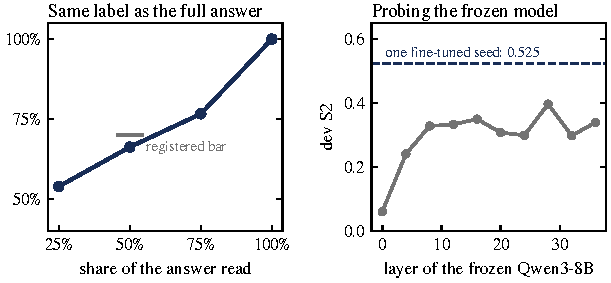
\includegraphics[width=0.78\textwidth,height=38mm,keepaspectratio]{figures/s_shortcut.pdf}\\[1mm]
  \raggedright\small
  \pred{half an answer agrees $\ge$70\% with the full-answer label} \quad\found{66\%} \failed\quad refusals show early, and General and Dodging only at the end.\\[0.8mm]
  \pred{a frozen-base probe reaches S2 $\ge$ 0.45} \quad\found{0.397} \failed\\[0.8mm]
  \pred{the probe is less question-bound than M1} \quad\found{same label on 45\% of disjoint siblings vs 19\%} \held
\end{frame}

\begin{frame}{E25: the register of hypotheses}
  \footnotesize
  \centering
  \renewcommand{\arraystretch}{1.2}
  \begin{tabular}{@{}l>{\raggedright\arraybackslash}p{0.56\textwidth}ll@{}}
    \toprule
     & Registered prediction & Result & Verdict \\
    \midrule
    a-1 & unrelated question: Clear-Reply share at least halves, $\le$50\% keep their label & 0.253 $\rightarrow$ 0.013, 19\% & \held \\
    b-1 & no stake (N): odds ratio $\ge 1.5$ & 1.18 & \failed \\
    b-2 & stake: P $-$ N $\ge +0.10$ & $-$0.031 & \failed \\
    b-3 & pursuit: $\ge$50\% of evasions become replies & 66\% & \held \\
    b-4 & notes: indirect $-$ non-answer $\ge +0.15$ & +0.113 & \failed \\
    c & half the answer: $\ge$70\% agree with the full label & 66\% & \failed \\
    d-1 & frozen-base probe: S2 $\ge$ 0.45 & 0.397 & \failed \\
    d-2 & probe repeats labels on $\ge$30\% of disjoint siblings & 45\% & \held \\
    \bottomrule
  \end{tabular}
\end{frame}

\begin{frame}{The metric and the 0.684 reference}
  \small
  \begin{itemize}\setlength{\itemsep}{1.5mm}
    \item A prediction is a true positive if \emph{any} annotator gave it. If every prediction is acceptable, macro-F1 = (classes predicted at least once) / 9: the score rewards landing in the reference set \emph{and} covering rare classes.
    \item Floors: always Explicit 0.060, uniform random 0.129, and TF-IDF + logistic regression 0.257.
    \item One annotator scored against the other two reaches 0.684. That is a \textbf{two-annotator} score, and our dev numbers use three annotators per item, which is easier. In the two-annotator regime, the first-scoring accuracy point (0.669) scores 0.589.
    \item The test set has two annotators per item, shorter answers (median 59 vs 292 words) and transcript artifacts.
  \end{itemize}
\end{frame}

\begin{frame}{Implementation details}
  \footnotesize
  \begin{columns}[T,onlytextwidth]
    \begin{column}{0.5\textwidth}
      \textbf{M1 and students}: Qwen3-8B-Base, bf16; LoRA $r = 16$, $\alpha = 32$, dropout 0.05 on all attention and MLP projections, and a new 9-way head on the last token. Training uses AdamW at $10^{-4}$, a cosine schedule, 5\% warm-up, batch 16 and 12 epochs, keeping the epoch with the best slice macro-F1. The input is ``Sub-question / Full question'' ($\le$256 tokens) plus the answer, $\le$1,024 in all. Students use the same recipe with a soft-target loss on $\tfrac12$ gold $+ \tfrac12 q$.
      \vspace{2mm}

      \textbf{M3}: Qwen3.8-27B-FP8 with vLLM, thinking off, one output token and top-20 log-probabilities. The prompt holds the task, 9 definitions, a confusion guide, the item and 4 lettered candidates, and $q$ is averaged over 4 cyclic orders.
    \end{column}
    \begin{column}{0.47\textwidth}
      \textbf{Frozen instrument} (\texttt{frozen\_system.json}): 10 seeds, slice calibration $\tau_C = 0.20$ and $T = 2.15$, top-4 candidates, and deferral iff $u \ge 0.638$ (slice 70\% quantile). Kept items use $\tau_1 = 1.15$, deferred items $\lambda = 0.5$ and $\tau = -0.55$. It reproduces the E23 predictions exactly.
      \vspace{2mm}

      \textbf{Protocol}: epochs, calibration and thresholds are set on a fixed 345-row train slice, dev-fitted parameters by 5-fold nested CV, with 10 paired seeds per claim. Registered hypotheses and time-stamped amendments are in \texttt{docs/experiment\_log.md}.
    \end{column}
  \end{columns}
\end{frame}
